\documentclass{ltugproc}

\usepackage[hybrid]{markdown}
\newcommand\term[1]{\textit{#1}}
\newcommand\command[1]{\texttt{#1}}
\newcommand\packagename[1]{\texttt{#1.sty}}
\newcommand\option[1]{\texttt{-\/-#1}}
% \usepackage{microtype}
\newcommand\texfourht{\term{\TeX4ht}}
\newcommand\texfourhtcmd{\command{tex4ht}}
% \newcommand\DVI{\acro{DVI}}

\newcommand\nazev[1]{#1}
\newcommand\parencite[1]{#1}
\newcommand\prikaz[1]{\texttt{#1}}
\newcommand\prepinac[1]{\texttt{-\/-#1}}

\author{Michal Hoftich}
\title{\texfourht: LaTeX to Web publishing}
\address{Charles University, Faculty of Education}
\netaddress{michal.hoftich@pedf.cuni.cz}
\personalURL{https://www.kodymirus.cz}
\begin{document}

\begin{abstract}
  TODO: add abstract
\end{abstract}
\maketitle

\section{Overview of the conversion process}
\texfourht\ is a system for conversion of \TeX\ documents to various output
formats. Most notably \HTML, or \term{OpenDocument Format}, supported by word processors such as Microsof Word or LibreOffice
Writer. 



The package \packagename{tex4ht} starts the conversion process. It loads special 
configuration files for packages supported by \texfourht. These configuration
files serve may fix clashes between the configured package and \texfourht, but most
notably the package commands can be patched to insert special marks to the \DVI\ file, so-called
hooks. These hooks are then populated with tags in the selected output format. 

The generated \DVI\ file is then processed with the \texfourhtcmd\ command.



\begin{figure*}[hbt!]
  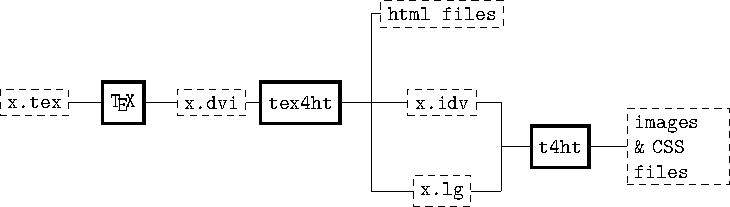
\includegraphics[width=\textwidth]{img/tex4ht_process.pdf}
\caption{\texfourht\ process overview}
\label{fig:overview}
\end{figure*}


Tento článek navazuje na předchozí příspěvek autora ve \nazev{Zpravodaji}
\parencite{hoftich:16}, který byl zaměřený na problematiku tvorby
elektronických knih, ovšem byly v~něm také
představeny postupy využívané konverzním systémem \nazev{TeX4ht} pro konverzi
z~\TeX u do výstupních formátů a nastíněna problematika samotné konverze z~\TeX u
do formátů založených na značkovacím jazyce XML. 
Nyní se zaměříme na některé nové vlastnosti sestavovacího programu pro \nazev{TeX4ht} jménem
\prikaz{make4ht} a pokročilejší možnosti konfigurace podoby výstupních souborů.

Připomeňme si však některé základní informace. \nazev{TeX4ht} je konverzní
systém který je založený na vkládání instrukcí výstupního formátu přímo při
překladu dokumentu \TeX em. Výsledkem kompilace je DVI soubor, který je
následně zpracován příkazem \prikaz{tex4ht}. Ten vytvoří výsledné XML soubory a
speciální soubory s~příponami \nazev{.idv} a \nazev{.lg}.
První z~nich obsahuje DVI kód, ze kterého mají být vytvořeny obrázky
(v~základním nastavení například matematická prostředí). Druhý je řídící soubor
pro poslední příkaz, \prikaz{t4ht}. Ten je využíván pro konverzi obrázků
z~\nazev{.idv} souboru, volání externích příkazů, nebo vytvoření hlavního CSS
souboru.

V~předchozím odstavci jsme použili výraz \nazev{TeX4ht} ve dvou různých
významech. Jednak jako název celého konverzního systému, jednak jako jednu
z~částí tohoto systému, která zpracovává DVI soubor. Existuje ještě další součást
systému s~tímto názvem, balíček \TeX ových maker \prikaz{tex4ht.sty}, který
zajišťuje vkládání XML značek do výstupního dokumentu.

\section{Sestavovací program \prikaz{make4ht}}

Jak do tohoto schématu zapadá \prikaz{make4ht}? Protože se celý konverzní proces
skládá z~několika na sebe navazujících kroků, vyžívají se pro kompilaci
systémem \nazev{TeX4ht} skripty, které tento proces ulehčují. Existuje jich
celá řada, liší se v~podporovaném výstupním formátu a použitém \TeX ovém enginu
a formátu. Nejznámější z~nich je \nazev{htlatex}, který využívá engine pdf\TeX\
s~formátem \LaTeX{} a produkuje výstup ve formátu HTML. Skripty zajišťují načtení
balíčku s~makry \prikaz{tex4ht.sty} bez nutnosti jeho použití
v~konvertovaném dokumentu.

Tyto skripty jsou ovšem neflexibilní, každé jejich spuštění provede
trojnásobnou kompilaci dokumentu \TeX em. To zajistí správnou strukturu
hypertextových odkazů a tabulek, ty totiž vyžadují několikanásobnou kompilaci
pro svojí správnou funkci. V~následujících krocích je dokument zpracován
\prikaz{tex4ht} a \prikaz{t4ht}. Pokud dokument obsahuje například seznam
literatury nebo zkratek, které jsou vytvářeny externími programy, je třeba
zavolat nejdříve \prikaz{htlatex}, poté požadovaný program a poté opět
\prikaz{htlatex}. V~případě větších dokumentů může být čas potřebný pro
kompilaci tímto způsobem poměrně dlouhý.

\prikaz{make4ht} umožňuje tvorbu sestavovacích skriptů v~jazyce \nazev{Lua}, ve
kterých lze volat externí příkazy podle potřeby. S~pomocí takzvaných
\nazev{módů} lze ovlivnit pořadí kompilace pomocí přepínačů přímo z~příkazové
řádky. Například základní skript používaný \prikaz{make4ht} podporuje
\nazev{draft} mód, který spustí pouze jednu kompilaci dokumentu, místo
obvyklých tří. Toho se dá využít pro zrychlení kompilace v~případě, kdy se
v~dokumentu od poslední kompilace nezměnily křížové odkazy a pouze chceme získat
rychlý náhled na jeho současnou podobu.

Původně byl \prikaz{make4ht} součástí systému \nazev{TeX4ebook}, kde zajišťoval
podporu pro sestavovací skripty, postupně se z~něj však oddělil a v~současné
době plně nahradil staré skripty používané pro konverzi systémem \nazev{TeX4ht}. 
Kromě podpory pro sestavovací skripty také umožňuje snadný výběr \TeX ového
engine použitého pro kompilaci, volbu výstupního formátu, podporu pro kódování
Unicode ve výstupních souborech a další vlastnosti.

V~současné době je podporován pouze \LaTeX, podpora pro Plain\TeX\ je
komplikovanější a Con\TeX{}t podporován není. V~následujícím textu
se zaměříme pouze na \LaTeX.

\subsection{Volby \prikaz{make4ht} pro příkazovou řádku}

\prikaz{make4ht} podporuje řadu přepínačů a voleb, které ovlivňují průběh kompilace a zpracování výstupních souborů. \prikaz{make4ht} může být spuštěn tímto způsobem:

\begingroup
\small
\begin{verbatim}
make4ht [přepínače pro make4ht] soubor.tex "volby pro tex4ht.sty" \
"přepínače pro tex4ht" "přepínače pro t4ht" "přepínače pro TeX"
\end{verbatim}
\endgroup

Tento komplikovaný způsob vychází z~fungování \prikaz{htlatex} a ostatních
starých skriptů, které řešily nutnost předávání voleb pro všechny komponenty
zapojené v~kompilaci. Ve většině případů naštěstí není třeba této možnosti
využívat, většinu vlastností, které poskytují \prikaz{tex4ht} a \prikaz{t4ht}
lze vyžádat pomocí přepínačů pro \prikaz{make4ht}.

Všechny přepínače, které \prikaz{make4ht} podporuje, mají krátkou a dlouhou
verzi. Krátké přepínače lze navíc spojovat dohromady. Následující dva příkazy
jsou totožné:

\begin{verbatim}
make4ht --lua --utf8 --mode draft clanek.tex
make4ht -lum draft clanek.tex
\end{verbatim}

Tento příkaz využije Lua\LaTeX{} pro kompilaci, která proběhne pouze jednou díky
využití \nazev{draft} módu, a výsledný dokument bude v~textovém kódování UTF-8.
Volby pro přepínače jsou od nich odděleny mezerou.

Kromě přepínačů \prepinac{lua}, \prepinac{utf8} a \prepinac{mode} existuje ještě řada dalších užitečných přepínačů:

\begin{description}
  \item[\prepinac{config (-c)}] konfigurační soubor pro \nazev{TeX4ht}. Umožňuje uživatelsky změnit značky vkládané do výstupních souborů.
  \item[\prepinac{build-file (-e)}] sestavovací soubor.
  \item[\prepinac{output-dir (-d)}] adresář, do kterého budou zkopírovány výstupní soubory.
  \item[\prepinac{shell-escape (-s)}] použije volbu \verb|--shell-escape| pro \LaTeX, bude tedy možné spouštět z~něj externí příkazy.
  \item[\prepinac{xetex (-x)}] dokument bude kompilován pomocí Xe\LaTeX u.
  \item[\prepinac{format (-f)}] volba výstupního formátu a rozšíření.
\end{description}

Existují ještě další přepínače, ale tyto jsou nejužitečnější pro běžné využití.

\subsection{Výstupní formáty a rozšíření}

\nazev{TeX4ht} podporuje širokou škálu formátů založených na XML, od XHTML,
přes ODT až po DocBook a TEI. Zájem uživatelů je však zaměřen prakticky pouze
na varianty HTML a OpenDocument Format, který 
je podporován textovými procesory jako je LibreOffice nebo MS Word.

Přepínač \prepinac{format} tedy podporuje pouze následující formáty: html5,
xhtml a odt (je třeba využít malá písmena). Přednastaveným formátem je HTML5.
Ostatní formáty, jako je DocBook, lze vybrat pomocí volby pro \prikaz{tex4ht.sty}:

\begin{verbatim}
make4ht filename.tex "docbook"
\end{verbatim}



V~přepínači \prepinac{format} lze také načíst rozšíření.  Rozšíření umožňují ovlivnit kompilaci
bez nutnosti použít sestavovací skript. 
Seznam využitých rozšíření lze zapsat za název formátu, zapínají se pomocí
znaku plus, pomocí znaku mínus lze rozšíření zakázat\footnote{Rozšíření lze
  zapnout i ze sestavovacího skriptu, takové rozšíření je poté možné vypnout
z~příkazové řádky.}. Následující příkaz využije příkaz \prikaz{HTML Tidy} pro
opravení některých běžných chyb ve vygenerovaném HTML souboru:

\begin{verbatim}
make4ht -f html5+tidy simple-example.tex
\end{verbatim}

Dostupná jsou následující rozšíření:

\begin{description}
  \item[\texttt{latexmk\_build}] využije příkaz \prikaz{latexmk} pro sestavení
    dokumentu. Ten se postará o~volání externích příkazů, například pro tvorbu
    seznamu literatury.
  \item[\texttt{tidy}] vyčistí HTML soubor pomocí příkazu \prikaz{tidy}.
  \item[\texttt{dvisvgm\_hashes}] efektivní generování obrázků pomocí příkazu
    \prikaz{dvisvgm}. Dokáže využít více procesorových jader a vytváří pouze
    obrázky, které byly změněny nebo vytvořeny od poslední kompilace. Tím
    dochází ke znatelnému zrychlení kompilace.
  \item[\texttt{common\_filters} {\normalfont a} \texttt{common\_domfilters}]
    vyčistění dokumentu pomocí filtrů. Filtrům se budeme věnovat dále v~textu.
  \item[\texttt{mathjaxnode}] konverze matematického kódu ve formátu MathML do
    speciálního HTML za využití projektu \nazev{MathJax Node
    Page}\footnote{\url{https://github.com/pkra/mathjax-node-page/}}. Díky tomu
    lze zobrazit kvalitně matematiku i ve webových prohlížečích bez podpory
    MathML, bez nutnosti využít JavaScript.
    % příklad https://www.kodymirus.cz/samples/mathjaxnode/maths.html
  \item[\texttt{staticsite}]  vytvoří dokument použitelný pro generátory statických
    stránek, jako je například
    \nazev{Jekyll}\footnote{\url{https://jekyllrb.com/}}. Ty jsou využitelné
    například pro tvorbu blogu.
\end{description}

Rozšíření je možné dále konfigurovat.
Tím se dostáváme ke konfiguračnímu souboru a sestavovacím skriptům.

\subsection{Konfigurační soubor pro \prikaz{make4ht}}

\prikaz{make4ht} podporuje sestavovací skripty v~jazyce Lua. Jejich pomocí je
možné volat externí příkazy v~průběhu kompilace, předávat jim parametry,
používat filtry na výstupní soubory, ovlivňovat konverzi obrázků nebo
konfigurovat rozšíření.

Konfigurační soubor \texttt{.make4ht} je speciální sestavovací skript, který je
načítaný automaticky a měl by obsahovat pouze obecné konfigurace. Oproti tomu
normální sestavovací soubory mohou obsahovat konfigurace platné pro daný
dokument. Konfigurační soubor může být umístěný v~adresáři s~dokumentem, nebo
v~jeho nadřazených adresářích. To je užitečné například pokud bychom tvořili
blog, kde každý dokument je umístěný ve vlastním adresáři. V~nadřazeném
adresáři může být umístěný konfigurační soubor, který zajistí správné
zpracování. Zde je drobný příklad:

\begin{verbatim}
filter_settings "staticsite" {
  site_root = "output" 
}

Make:enable_extension("common_domfilters")
if mode=="publish" then
  Make:enable_extension("staticsite")
  Make:htlatex {}
end

\end{verbatim}

Tento konfigurační soubor nastavuje volbu \texttt{site\_root} pro rozšíření
\nazev{staticsite} pomocí příkazu \verb|filter_settings|. Pomocí tohoto příkazu
lze nastavit volby pro filtry, ale také rozšíření. Název filtru nebo rozšíření
je oddělený od příkazu mezerou, poté následuje další mezerou oddělené pole, ve
kterém lze nastavit volby daného filtru. Oproti běžným konvencím příkazů
v~jazyce Lua zde nevyužíváme uvozovky jako u~běžných funkcí!

Dalším použitým příkazem je \verb|Make:enable_extension|, který povolí
rozšíření. V~tomto případě je rozšíření \texttt{common\_domfilters} použito pro
každou kompilaci, ovšem rozšíření \texttt{staticsite} pouze v~módu
\nazev{publish}, čehož je dosaženo podmínkou \verb|mode=="publish"|.

Příkaz \verb|Make:htlatex {}| vynutí jednu kompilaci \LaTeX em. 

Nyní lze spustit \prikaz{make4ht} v~módu \nazev{publish}: 

\begin{verbatim}
make4ht -um publish simple-example.tex
\end{verbatim}

Bude vytvořen adresář \nazev{publish}, pokud již neexistuje, do kterého budou
zkopírovány HTML a CSS soubory ve formátu \textit{datum publikace-originální
název}. Statické generátory většinou očekávají názvy souborů v~tomto formátu,
čímž se zajistí chronologické řazení stránek.

Výsledný HTML soubor může mít následující podobu:

\begin{verbatim}
---
time: 1544811015
date: '2018-12-14 18:10:47'
title: 'sample'
styles:
- '2018-12-14-simple-example.css'
meta:
- charset: 'utf-8'
---
<p>Sample document</p>
\end{verbatim}


Hlavička dokumentu uzavřená mezi dvojicí \verb|---| obsahuje proměnné ve
formátu YAML extrahované z~HTML souboru, ze kterého zůstal pouze základní text.
Statický generátor poté může vytvořit stránku na základě šablony a proměnných
v~hlavičce. 

Toto byl pouze základní příklad, filtry a rozšíření mají mnohem širší možnosti
nastavení, všechny volby jsou popsány v~dokumentaci \prikaz{make4ht} \parencite{make4ht}.


\subsection{Sestavovací skripty}


V~sestavovacích skriptech můžeme využívat stejné postupy jako v~konfiguračním
souboru, ale více zaměřené na konkrétní kompilovaný dokument. Příklad
sestavovacího skriptu byl představen v~předešlém článku \parencite[s.
95]{hoftich:16}, ukážeme si zde tedy pouze novou vlastnost, kterou jsou DOM
filtry. Ty využívají možností knihovny LuaXML \parencite{luaxml}, která
umožňuje zpracovávat XML soubory pomocí rozhraní \nazev{Document Object Model (DOM)}.
Díky tomu lze snadno procházet elementy, upravovat je, vytvářet nebo
odstraňovat.

Využití DOM filtrů si ukážeme na příkladu určeném pro Lua\LaTeX: 

\begin{verbatim}
\documentclass{article}
\begin{document}
Test {\itshape háčků}
\end{document}
\end{verbatim}

Kvůli známé chybě při zpracování DVI souboru příkazem \prikaz{tex4ht} bude
vytvořen HTML soubor, kde každý znak s~diakritikou bude umístěn v~samostatném
elementu:

\begin{verbatim}
<!--l. 4--><p class="noindent" >Test <span 
class="rm-lmri-10">h</span><span 
class="rm-lmri-10">á</span><span 
class="rm-lmri-10">čk</span><span 
class="rm-lmri-10">ů</span> </p> 
\end{verbatim}


Následující sestavovací soubor toto napraví pomocí vestavěného DOM filtru
\nazev{joincharacters}. Navíc změníme atribut \nazev{class} všech elementů
\verb|<p>| na hodnotu \nazev{mypar}, abychom si ukázali práci s~DOM rozhraním:

\begin{verbatim}
local domfilter = require("make4ht-domfilter")

local function domsample(dom)
  -- následující příkaz projde 
  -- všechny elementy <p>
  for _, par in ipairs(dom:query_selector("p")) do
    -- nastavit atribut "class"
    par:set_attribute("class", "mypar")
  end
  return dom
end

local process = domfilter({"joincharacters", domsample})
Make:match("html$", process)
\end{verbatim}


Skript využívá standardní funkci jazyka Lua \verb|require| k~načtení knihovny
\verb|make4ht-domfilter|. To vytvoří funkci \verb|domfilter|, která má jako
parametr seznam DOM filtrů, které se mají vykonat. Každé volání funkce \verb|domfilter|
vytvoří další funkci, která může být využita jako parametr pro funkci
\verb|Make:match|. Parametry v~poli mohou být buď název existujícího DOM
filtru, nebo funkce definovaná v~sestavovacím souboru. 
Funkce \verb|process| bude spuštěna na každém souboru jehož název končí na
\verb|html|.

Výsledný HTML soubor nyní neobsahuje nadbytečné elementy \verb|<span>| a
element \verb|<p>| má hodnotu atribut \nazev{class} nastavenu na \nazev{mypar}:

\begin{verbatim}
<!-- l. 3 --><p class='mypar'>
Test <span class='rm-lmri-10'>háčků</span> 
</p> 
\end{verbatim}


\section{Konfigurace TeX4ht}

Od \prikaz{make4ht} nyní přejděme ke konfiguraci \nazev{TeX4ht} jako takového.
Značky výstupního formátu vkládané do dokumentu jsou plně konfigurovatelné
pomocí několika mechanismů. Nejjednodušší je využití voleb balíčku
\prikaz{tex4ht.sty}, větší možnosti nastavení nabízí konfigurační soubor a
nejpokročilejší pak \nazev{4ht} soubory.

Při kompilaci \TeX ového souboru pomocí \prikaz{make4ht} nebo jiného
kompilačního skriptu se ještě před načtením samotného dokumentu načte balíček
\prikaz{tex4ht.sty}.  Volby balíčku jsou získány z~argumentů kompilačního
skriptu. Díky tomu není třeba vkládat balíček \prikaz{tex4ht.sty} v~samotném
dokumentu.

Mechanismus načítání souborů je upraven tak, aby se každý načítaný soubor
registroval do \nazev{TeX4ht}. Pro některé balíčky \nazev{TeX4ht} také obsahuje
kód, který zabraňuje jejich načítání, nebo okamžitě předefinovává některá
makra. To je nezbytné pro balíčky, které jsou s~\nazev{TeX4ht} nekompatibilní,
jako je například \nazev{Fontspec}. 

Po vykonání \nazev{preamble} dokumentu se načítají konfigurační soubory pro balíčky
detekované při jejím zpracování. Tyto soubory mají název \texttt{jméno souboru
bez přípony + .4ht}. Jejich hlavní funkcí je vkládat konfigurovatelná makra,
takzvané háčky, do příkazů poskytovaných balíčkem. Obecně je lepší makra
nepředefinovávat, ale pouze záplatovat pomocí příkazů, které pro tento účel
\nazev{TeX4ht} poskytuje.

Po zpracování konfiguračních souborů pro balíčky se načítají konfigurační
soubory výstupního formátu. Ty definují obsah konfiguračních maker, háčků.
Především se do nich vkládají značky výstupního formátu, ale mohou obsahovat
libovolné příkazy. Je možná také podmíněná konfigurace na základě voleb balíčku
\prikaz{tex4ht.sty}. Každý konfigurační soubor výstupního formátu může testovat
libovolnou volbu, z~čehož vyplývá, že neexistuje jejich konečný seznam a pro
každý formát existují jiné volby.

\subsection{Volby balíčku \texttt{tex4ht.sty}}

Protože se nedoporučuje vkládat balíček \prikaz{tex4ht.sty} přímo do dokumentu,
je možné předat mu volby jiným způsobem. Nejjednodušším je pomocí argumentu pro
kompilační skript. Vždy je to argument následující po názvu dokumentu:

\begin{verbatim}
make4ht filename.tex "mathml,mathjax"
\end{verbatim}

Volby použité v~tomto případě jsou \nazev{mathml} a \nazev{mathjax}. Další
možností předání voleb je předání pomocí příkazu \verb|\Preamble| v~soukromém
konfiguračním souboru, který si ukážeme v~další sekci.

Jak již bylo řečeno, neexistuje konečný seznam voleb, každý výstupní formát
může podporovat jejich libovolné množství.

Můžeme si ovšem ukázat některé volby, které se týkají matematických výstupů v~HTML.
Normální konfigurace pro matematická prostředí produkuje směs formátovaného
textu a obrázků pro složitější výstupy, které nejdou snadno vytvořit pomocí HTML elementů.
Někdy tato vlastnost nevypadá dobře. Jako alternativu lze použít obrázky pro
veškerý matematický obsah. Toho lze dosáhnout pomocí voleb \nazev{pic-m} pro
inline matematiku a \nazev{pic-název prostředí} pro matematická prostředí,
například \nazev{pic-align}.

Normálně jsou obrázky vytvářeny ve formátu PNG. Vyšší kvality lze dosáhnout
s~využitím vektorového formátu SVG. Ten může být vynucen pomocí volby
\nazev{svg}.

Dokumentace \nazev{TeX4ht} je poměrně spartánská. Obsáhlejší informace
o~konfiguraci příkazů lze nalézt v~log souboru vytvořeném při kompilaci dokumentu
s~pomocí volby \nazev{info}.

Volby uvedené v~prvním příkladu, \nazev{mathml} a \nazev{mathjax} poskytují
obecně nejlepší výstup matematického obsahu. Značkovací jazyk MathML umožňuje
zakódovat matematické informace, jeho podpora ve webových prohlížečích je však
špatná. S~využitím knihovny
\nazev{MathJax}\footnote{\url{https://www.mathjax.org/}} je možné jej zobrazit
ve všech moderních prohlížečích s~podporou jazyka JavaScript.

Samotná volba \nazev{mathjax} bez \nazev{mathml} úplně vypne zpracování
matematiky při kompilaci, veškerý matematický obsah zůstane v~HTML dokumentu
jako \TeX ová makra. \nazev{MathJax} poté dokument zpracuje a vykreslí
matematiku správným způsobem. Nevýhodou tohoto způsobu je, že \nazev{MathJax}
nepodporuje všechny balíčky a uživatelské příkazy. 


\subsection{Soukromý konfigurační soubor}

Pomocí soukromého konfiguračního souboru je možné vkládat vlastní obsah do
konfiguračních háčků. Tento soubor má zvláštní strukturu:

\begin{verbatim}
...Definice v~preamble...
\Preamble{volby pro tex4ht.sty}
... Normální konfigurace ...
\begin{document}
... Konfigurace pro hlavičku HTML souboru
\EndPreamble
\end{verbatim}

Příkazy \verb|\Preamble|, \verb|\begin{document}| a \verb|\EndPreamble| musí
být v~konfiguračním souboru obsaženy. Cesta k souboru může být předána
\nazev{make4ht} pomocí parametru \verb|-c|:

\begin{verbatim}
make4ht -c myconfig.cfg filename.tex
\end{verbatim}

Pokud konfigurační soubor není uložený v~aktuálním pracovním adresáři, je nutno
použít plnou cestu k souboru.


Existuje několik konfiguračních příkazů. Nejdůležitějším je \verb|\Configure|,
který nastavuje běžné konfigurace, dalšími jsou například \verb|\ConfigureEnv|
pro nastavení prostředí, nebo \verb|\ConfigureList| pro seznamy.

Příkaz \verb|\HCode| se používá pro vkládání značek výstupního formátu.
Součástí jeho argumentu může být příkaz \verb|\Hnewline| pro vložení zalomení
řádku. Instrukce \verb|\Css| vloží kód pro kaskádové styly do CSS souboru.


Následující ukázka použije element \verb|<em>| pro příkaz \verb|\textit|:

\begin{verbatim}
\Configure{textit}{\HCode{<em>}\NoFonts}{\EndNoFonts\HCode{</em>}}
\end{verbatim}

Příkaz \verb|\Configure| podporuje variabilní počet argumentů, záleží na
definici háčků, kolik argumentů je potřeba. Prvním argumentem je vždy název
konfigurace, další argumenty poté vkládají kód do háčků. V~typickém případě
vyžaduje konfigurace dva háčky -- jeden umístí kód před začátek příkazu, druhý
za jeho konec. Tak je tomu v~případě konfigurace pro \texttt{textit}. Název
konfigurace se může shodovat s~názvem konfigurovaného příkazu, jako v~tomto
případě, ale vždy záleží na konfiguračním \nazev{4ht} souboru pro daný balíček,
jaký název použije.


Příkaz \verb|\NoFonts| zakáže vkládání formátovacích elementů při zpracování
DVI souboru. \prikaz{tex4ht} vkládá automaticky tyto elementy při změně písma.
Díky tomu je možné vytvořit základní formátování i pro nepodporované příkazy
bez konfigurací, ovšem pro konfigurované příkazy je toto zbytečné. 



Komplikovanou problematikou jsou odstavce. \nazev{TeX4ht} je někdy vkládá na
nevhodná místa. Týká se to především konfigurací prostředí, která mohou
obsahovat několik odstavců a celý svůj obsah umísťují do jednoho elementu. Může
se stát, že počáteční značka odstavce je umístěna před začátkem tohoto elementu,
správně by ovšem měla následovat až po něm. Pro tento případ existují příkazy
\verb|\IgnorePar|, který zabrání vložení značky pro následující odstavec, a
\verb|\EndP|, který vloží zavírací značku pro předešlý odstavec. Existuje více
příkazů pro práci s~odstavci, ale tyto jsou nejdůležitější.

V~následujícím příkladu použijeme hypotetické prostředí \texttt{rightaligned},
které by mělo být umístěno v~elementu \verb|<article>|. 

\begin{verbatim}
\ConfigureEnv{rightaligned}
{\HCode{<section class="right">}}
{\HCode{</section>}}{}{}
\end{verbatim}

Příkaz \verb|\ConfigureEnv| očekává pět parametrů, prvním je název
konfigurovaného prostředí, druhým je kód vložený na začátku prostředí a třetím
kód vložený na jeho konci. Zbylé dva argumenty se používají pouze pokud je
konfigurované prostředí založeno na seznamu, ve většině případů mohou zůstat prázdné. 
HTML kód vytvořený touto konfigurací může vypadat následovně:

\begin{verbatim}
<p class="indent" >   <section class="right">
...
</p><p class="indent></section>
\end{verbatim}

Tento kód je nevalidní, protože ukončovací značka pro element \verb|<p>| je
umístěna na špatné úrovni zanoření. Nevalidní kód může způsobit přerušení běhu
DOM filtrů a jiných nástrojů, které zpracovávají výsledné XML soubory. Této
situaci je třeba předcházet.

Správná konfigurace je poněkud komplikovanější:


\begin{verbatim}
\ConfigureEnv{rightaligned}
{\ifvmode\IgnorePar\fi\EndP\HCode{<section class="right">}\par}
{\ifvmode\IgnorePar\fi\EndP\HCode{</section>}}{}{}
\end{verbatim}

V~tomto případě řídíme vkládání značek pro odstavce sami a výsledek je v~pořádku:


\begin{verbatim}
<section class="right">
<!--l. 9--><p class="indent" >
...
</p></section>
\end{verbatim}

V~konfiguracích můžeme také vyžádat konverzi části dokumentu na obrázek. Toho
se dá docílit pomocí příkazů \verb|\Picture*|, respektive \verb|\Picture+|.
Rozdíl mezi nimi je ten, že první zpracovává svůj obsah jako vertikální box.
V~každém případě se obsah mezi těmito příkazy a ukončovacím příkazem
\verb|\EndPicture| převede na obrázek.

Těchto příkazů lze využít například pro konverzi složitější matematiky nebo diagramů,
ale čistě technicky podporují veškerý obsah, který dokáže zpracovat použitý
konvertor z~DVI do obrazových souborů, typicky \nazev{Dvipng} nebo
\nazev{Dvisvgm}.

Následující příklad vytvoří obrázek pro text obsažený v prostředí \nazev{topicture}:

\begin{verbatim}
\documentclass{article}
\newenvironment{topicture}{\bfseries}{}
\begin{document}
\begin{topicture}
Obsah tohoto prostředí by měl být zobrazen jako obrázek
\end{topicture}
\end{document}
\end{verbatim}

Konfigurace pro prostředí \nazev{topicture} využije příkazu \verb|\Picture*|:

\begin{verbatim}
\ConfigureEnv{topicture}{\Picture*{}}{\EndPicture}{}{}
\end{verbatim}


\section{Závěr}

Možnosti konfigurace \nazev{TeX4ht} jsou rozsáhlé, v~předešlém textu jsme se
dotkli pouze základů, které by však měly vystačit pro řešení nejběžnějších
otázek, které uživatelé tohoto systému řeší. Vynechali jsme také ukázky, jakým
způsobem lze přidat konfiguraci pro nový \LaTeX ový balíček. Tato témata by
vydala na rozsáhlé samostatné články.

Díky sestavovacímu systému \prikaz{make4ht} je použití celého systému snazší a
efektivnější než tomu bylo v~minulosti.

V~současné době probíhá za finanční podpory poskytnuté \nazev{Českoskovenským
sdružením uživatelů \TeX u} tvorba nové dokumentace pro \nazev{TeX4ht}, kde
budou témata tohoto článku probrána do větší hloubky, spolu s~konkrétními
příklady užití. 


\printbibliography
\begin{summary}

  The article gives overview of the current state of development of TeX4ht,
  \LaTeX\ to XML convertor. It introduces \prikaz{make4ht}, a build system for
  TeX4ht as well as basic ways how to configure TeX4ht.

\end{summary}


\end{document}
